\documentclass[12pt]{article}
\usepackage[margin=2cm]{geometry}
\usepackage{amsmath}
\usepackage{graphicx}

\begin{document}

\noindent
The following muon table is from the Particle Data Group.\footnote{\tt https://pdg.lbl.gov/2020/listings/rpp2020-list-muon.pdf}

\begin{center}
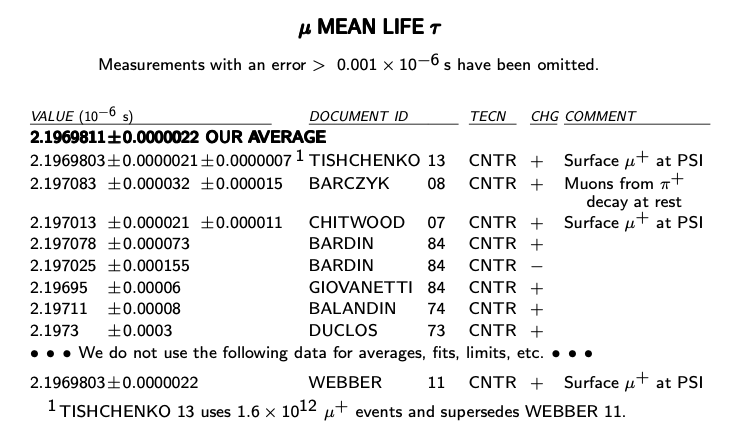
\includegraphics[scale=0.5]{muon-mean-life.png}
\end{center}

\noindent
Let us compute muon decay time from theory and compare it to the average measured value of 2.1969811 microseconds.

\bigskip
\noindent
The result from QED theory is the following formula for muon mean life $\tau$.
\begin{equation*}
\tau=\frac{96\pi^2h}{G_F^2\left(m_\mu c^2\right)^5}
\end{equation*}

\noindent
$G_F$ is Fermi coupling constant, $m_\mu$ is muon rest mass.

\bigskip
\noindent
From NIST\footnote{\tt https://physics.nist.gov/cuu/Constants/index.html} we have
\begin{align*}
G_F&=1.1663787\times10^{-5}\;\text{GeV}^{-2}
\\
m_\mu&=1.883531627\times10^{-28}\;\text{kilogram}
\\
h&=6.62607015\times10^{-34}\;\text{joule}\;\text{second}\;\text{(exact)}
\\
c&=299792458\;\text{meter}\;\text{second}^{-1}\;\text{(exact)}
\\
1\,\text{eV}&=1.602176634\times10^{-19}\;\text{joule}\;\text{(exact)}
\end{align*}

\noindent
Hence
\begin{equation*}
\tau=2.18735\times10^{-6}\,\text{second}
\end{equation*}

\noindent
The result is a bit smaller than the measured value.
\begin{equation*}
\frac{\tau}{2.1969811\times10^{-6}\;\text{second}}=0.9956
\end{equation*}

\end{document}
